%\section{Design Method}\label{sec:design_method}
This chapter shows focusses on each of the code generation phases and what our contributions are to this compiler. We describe how we have taken a compiler without support for explicit bypass registers, which is described in Section \ref{sec:basic_compiler_design} and improved, maintained and extended it. 

%Discuss maintaining, process of porting from llvm3.8 to LLVM4.0, and discuss new version LLVM5.0. Mention that this upgrade to 4.0 also drastically improved vectorization because the community develops this constantly. (maybe add example of CNN)

%TODO: move vectorization to here? Noooo.

\section{Back-end Code Generation}\label{sec:code_generation}
We will briefly discuss each of the code generation stages, which includes custom passes and standard passes supplied by the LLVM framework. Before generating code, we use LLVM's front-end to translate a high level language to an intermediate representation, called LLVM-IR. This can be further optimized and used as input for our back-end. We categorize the code generation phases in the back-end in three major categories.

\begin{figure}[H]
\centering
\hspace*{-.12in}
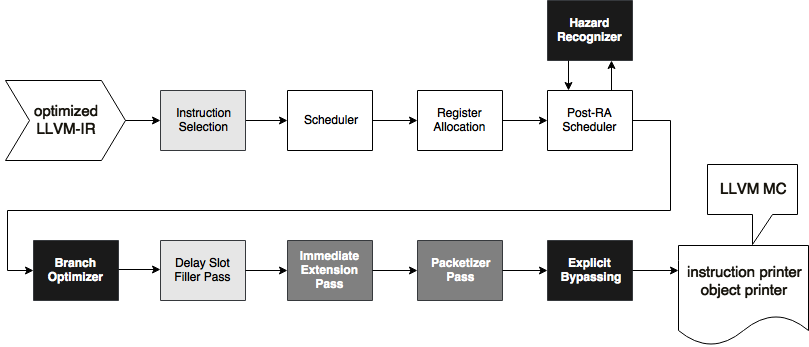
\includegraphics[scale=0.53]{figures/code_generation}
%TODO: change orange to yellow and yellow to orange in picture. 
\caption{Overview of the phases that the back-end is comprised of.}
\label{fig:simd_backend}
\end{figure}
%include an image with the pipeline having all these components.

%TODO: refere to problem where instr have no common operand, so it seems unrelated. 

%TODO: add text that explains the color, instruction selection is copied mostly from another architectures, and was already updated according to our architecture. / Hazard recognizer has partially been copied from other architectures, but was not suitable and has, therefore, been modified and tested. / Delay slot is a custom pass that was already implemented, but we have modified it to be more efficient. / Packetizer pass is as delivered, with a minor modification with hardly any efford.  / Bypass Regs is a custom pass that we developed during the duration of our work.

Firstly, we work on creating a schedule which is depicted in the top row of Figure \ref{fig:simd_backend}. The second row illustrates a collection of phases that do back-end specific transformations. Here we take care of special features that our architecture has. At last, now that we have code for our architecture, namely, an LLVM internal representation of it, we emit assembly or ELF object code (depicted in the rightmost part of the image) that our machine can understand.

%A list of all components that follow in the following section.
\begin{itemize}
	\item \textbf{Instruction Selection:} Uses a DAG, called \texttt{SelectionDAGs}, an abstraction for code representation suitable for phases ranging from Instruction Selection, Legalization to Lowering. Instruction selection is implemented in  \texttt{SimdISelDAGToDAG}, which is derived from \texttt{SelectionDAGISel} and consists of a bunch of transformations to transform specific instructions into instruction that are supported by our architecture. For example, transforming operations on immediate values with a value higher than one byte is partially implemented here. Lowering nodes of the directed acyclic graph (DAG) is done in \texttt{SimdISelLowering}, which is derived from \texttt{TargetLowering}. There the SIMD intrinsics and ISD instructions are lowered to Machine Instructions (MI) and sequences of MIs.
%\item \textbf{Scheduling:} Transforms a directed acyclic graph into an ordered list of instructions.
%\item \textbf{Register allocation:} Assigns physical registers to virtual registers of a list of instructions in SSA form.
	\item \textbf{Instruction Scheduler:} MIScheduler supplied by LLVM\\
MIScheduler is an instruction scheduler which supports VLIW scheduling. Considering there are two issue slots in this architecture, a VLIW scheduler would meet our requirements very well. One and two schedulers are defined for four stage pipeline and five stage pipeline respectively. The four stage pipeline scheduler is the default one while the five stage pipeline has the default one and additionally a post register allocation scheduler.
	\item \textbf{Register Allocation:} Greedy Allocator supplied by LLVM\\
	The Greedy allocator is a default allocator in LLVM. Since there is no special requirement to register allocation for now, the default allocator is enough to work. Apart from the default register allocator, there are more register allocators to choose from and it is possible to implement a custom register allocator.
	\item \textbf{Post Register Allocation Scheduler:} A second scheduling pass which we only need if we generate code for five stage pipeline configuration, otherwise, we disable it. The post RA scheduler uses a schedule hazard recognizer, which decides whether to prefer certain instruction over other instructions. For example, RaW hazards are detected and avoided by this algorithm.
	\item \textbf{Hazard Recognizer:} When the five stage pipeline is configured, consecutive instructions may have hazards. That is, when an instruction tries to read a register of which the result is not there yet because the operation took two cycles. This pass implements LLVM's \texttt{ScoreboardHazardRecognizer}, which we adapted to detect and resolve these hazards.
	%TODO: check implements / extends / derived
	\item \textbf{Delay Slot Filler:} For this architecture, jumps and branch instructions modify the program counter (PC) during the instruction decode stage. At that point, the instruction that follows the jump has already been fetched. The slot that follows a jump or branch instruction is called a delay slot. This pass aims to utilize delay slots by filling them with useful instructions.% that come after a jump or conditional branch instruction, i.e. instructions that modify the program counter.%VERIFY: `or e.g.?
	\item \textbf{Immediate Extension:} In principle, a one byte immediate value can be specified with an instruction. However, sometimes you may want to use a larger immediate. This pass allows us to use large immediates using \texttt{zimm} and \texttt{simm} instruction. These instructions have a 18 bit operand, that may be used for larger immediates.% will be a prefix of the original 8 bits  or using a shift to put a value in a register (up to 32 bits).
	\item \textbf{Packetizer:} Bundles scalar instructions with vector instructions. For each instruction it consults whether an issue slots is available on which the instruction can execute. This pass implements VLIW packetizer supplied by the LLVM framework.
	\item \textbf{Bypass Registers Allocation:} This pass exploits explicit data paths by allocating explicit registers to the generated code. This post-processing step can be replaced by one of the other approaches, which are discussed in Section \ref{sec:approaches}.
	\item \textbf{Instruction Printer:} MC is a sub-project of LLVM, which uses \texttt{MCInst} as a representation of an instruction, which is different from the code generator's existing notion of an instruction (\texttt{MachineInstr}). It is used during the last code generation stage when printing the instructions to a given output format. We further divide printing for different output formats, including binary format and SIMD assembly language in XAS-format. 
%TODO: move


\end{itemize}
The following sections give a more elaborate discussion on each custom pass and describes their relation to each other.

%TODO: validate and update
\section{Custom Passes}
This section describes the custom passes mentioned in the previous section. Dependencies and relations to other passes are described. After this, the linker, the assembler and the vectorizer are briefly discussed. The disassembler will not be implemented, but is also briefly described in this section.

\begin{table}[t!]
\caption{Relations between architecture design features and code generation phases.}
\begin{center}
\begin{tabular}{@{}l l l@{}}
\toprule
\textbf{Feature} & \textbf{Code Gen. Pass} \\ \hline
Hardware Pipeline 	& Delay Slot Filler 	& The delay slot, which is a product of the\\
				&				& pipeline is being filled with this pass.\\
			 	& Hazard Recognizer & Instructions do not always have single cycle\\
				&				 & latencies. This pass is necessary for a five\\
				&				& stage pipeline configuration. \\
Bit-width 			& Immediate Extension & With different data width, constants may be\\
				&				    & lowered in a different way. \\
ISA extension		& Instruction Selection & New instructions need to be described in\\
				&					& the back-end. \\
Operand bypassing 	& Bypass Register Allocation & This optional pass is developed to implement\\
				&					& explicit operand bypassing. It can be enabled\\
				&					& using compiler flag \texttt{-explicit}. \\
\bottomrule
\end{tabular}
\end{center}
\label{table:rel_feature_pass}
\end{table}%

\subsection{Hazard Recognizer}\label{sec:hazard_recogn}
When generating code for a four stage pipeline configuration, all instructions have a latency of one cycle. In that case, hazard recognition is not necessary.
In order to support code generation for a five stage pipeline configuration we have implemented a hazard recognizer. The hazard recognizer is used by the scheduler to determine if two consecutive instructions can be scheduled after each other. 

\lstset{style=customasm}
\begin{lstlisting}
addi r13, r0, 14
addi r12, r0, 10
mul r2, r5, r13  #latency=2
mul <@\textcolor{red!70!black}{r3}@>, r6, r12  #latency=2
add r2, r2, <@\textcolor{red!70!black}{r3}@>
\end{lstlisting}

We detect hazards by considering whether an operation has a RaW dependency with instruction that came prior to it. We have a true hazard when the instruction that came prior to it has a latency of more than one. The post register allocation (Post-RA) scheduler does a linear scan through the list of operation and queries the hazard recognizer whether an instruction can be scheduled. When it detects a hazard, it will consider other instructions that are ready to be scheduled and if there are none available without hazards, it will insert a no-op.

%It recognizes hazards by looking at whether the current instruction to be scheduled uses a register that is defined by the instruction issued in the previous cycle, which also has a latency of more than one cycle. If this is the case, we have a hazard and the instruction under consideration can not be scheduled in the current cycle. At this point we will consider other instructions that are ready to be scheduled and if there are none available without hazards, we will insert a no-op.
\subsection{Delay Slot Filler}
During the execution of a conditional branch or jump instruction the program counter (PC) is modified in the instruction decode (ID) stage. The proposed architecture has for any pipeline configuration, at least an instruction fetch (IF) and instruction decode (ID) stage, as we have discussed in Section \ref{sec:simd}. Therefore, during execution of the ID stage, the next instruction, with PC is PC+4 has already been fetched by the IF stage before the jump is executed. This slot will be executed before the instruction that the PC points at after modifying the PC and is called delay slot. %TODO: this paragraph can be shorter 

In order assure correct behaviour we intentionally 
%or initially (stood there in the first place)
place a no-op after each jump or branch instruction. However, sometimes we can do better. Namely we can use an instruction from before the jump instruction instead of a no-op. We search backwards to look at the previous two instructions and the instruction that comes after the jump, which are referred to as $prev_1$, $prev_2$ and $next$ respectively. When the backwards search does not fill the delay slot we intentionally insert a no-op, and if there is a vector operation that comes after the delay slot, we also need to insert a vector-nop, so that it will not be bundled with the delay slot later on by the packetizer.

%\captionof{lstlisting}{Fragment of assembly code to illustrate behaviour of the delay slot filler.}\label{lst:delayslot1}
%\begin{center}
%\hspace{2px}\begin{minipage}{.475\textwidth}
%\begin{lstlisting}[frame=tlrb]
%BB0_1:
%    sfne r1, 7
%    add r3, r3, r1
%    bf BB0_1
%    nop
%\end{lstlisting}
%\end{minipage}\hfill
%\begin{minipage}{.475\textwidth}
%\begin{lstlisting}[frame=tlrb]
%BB0_1:
%    sfne r1, 7
%    bf BB0_1
%    add r3, r3, r1
%   <@ @>
%\end{lstlisting}
%%\vspace{1.9em}
%\end{minipage}
%\end{center}

%Possibly scrap this case distinction 
%Add picture from scratch paper showing these cases

\captionof{lstlisting}{Fragment of assembly code to illustrate behaviour of the delay slot filler for the first case.}\label{lst:delayslot1}
\begin{center}
\hspace{2px}\begin{minipage}{.475\textwidth}
\begin{lstlisting}[frame=tlrb]
BB0_1:
    v.add r3, r6, r14
    v.add r4, r5, r12
    j BB0_1
    nop
\end{lstlisting}
\end{minipage}\hfill
\begin{minipage}{.475\textwidth}
\begin{lstlisting}[frame=tlrb]
BB0_1:
    v.add r3, r6, r14
    j BB0_1
    nop
    v.add r4, r5, r12
\end{lstlisting}
%\vspace{1.9em}
\end{minipage}
\end{center}

\begin{enumerate}
\item The ideal case is when the previous two instructions are both vector instructions. In that case, the vector instruction prior to the jump instruction can be moved to after it. Now the vector instruction that remains before the jump ($prev_1$) gets bundled with the jump instruction. If there was originally an instruction after to the jump instruction which is not a vector instruction, it would get bundled with the vector instruction that we moved by the packetizer pass. Therefore, we then need to insert a no-op to ensure the delay slot. %the instruction that came after is a scalar instruction, it would be merged with the filled instruction, therefore, in that case we need to add a nop, such that it bundles with the filled vector instruction.
\end{enumerate}

\captionof{lstlisting}{Fragment of assembly code to illustrate behaviour of the delay slot filler for the second case.}\label{lst:delayslot2}
\begin{center}
\hspace{2px}\begin{minipage}{.475\textwidth}
\begin{lstlisting}[frame=tlrb]
BB0_1:
    v.add r3, r6, r14
    v.add r4, r5, r12
    add r3, r3, r1
    j BB0_1
    nop
\end{lstlisting}
\end{minipage}\hfill
\begin{minipage}{.475\textwidth}
\begin{lstlisting}[frame=tlrb]
BB0_1:
    v.add r3, r6, r14
    j BB0_1
    add r3, r3, r1
    v.add r4, r5, r12
   <@ @>
\end{lstlisting}
%\vspace{1.9em}
\end{minipage}
\end{center}

\begin{enumerate}
\item[2] When the instruction before the jump ($prev_1$) is a scalar instruction with no dependencies to the jump itself, we can move it to the delay slot. We are now done if we moved a bundled instruction. Otherwise, when there are two vector operations prior to the jump instruction, we can again move one of them to to after the jump, and fully utilize the delay slot.

\item[3] We also consider the case where $prev_1$ is a vector instruction, and $prev_2$ is not a relational or jump instruction. Since the first case considers both $prev_1$ and $prev_2$ vector instructions, we consider cases where $prev_1$ is a vector and $prev_2$ is scalar operation by this case. %todo: little more in depth explanation of this pass
\end{enumerate}

\captionof{lstlisting}{Fragment of assembly code to illustrate behaviour of the delay slot filler for the third case.}\label{lst:delayslot3}
\begin{center}
\hspace{2px}\begin{minipage}{.475\textwidth}
\begin{lstlisting}[frame=tlrb]
BB0_1:
    add r3, r3, r1
    v.add r4, r5, r12
    j BB0_1
    nop
\end{lstlisting}
\end{minipage}\hfill
\begin{minipage}{.475\textwidth}
\begin{lstlisting}[frame=tlrb]
BB0_1:
    j BB0_1
    add r3, r3, r1
    v.add r4, r5, r12
   <@ @>
\end{lstlisting}
%\vspace{1.9em}
\end{minipage}
\end{center}
%todo: give case(s) that is not covered, followed by this line
The first two cases were already present, but required some modifications during upgrading to LLVM 4.0. We have added the third case because many delay slots were not being utilized.

%TODO: make case distinction here.
%\begin{enumerate}
%	 \item When the two operation before the jump instruction are both vector instructions,  
%\end{enumerate}
%TODO: make pseudo code of 

%Immediate extension 
\subsection{Immediate Extention}\label{sec:immediate_ext}
All immediate operations in Appendix \ref{appendix:i_type_instrs} have as last operand, a one byte immediate. However, sometimes we need larger numbers. Therefore, we lower constants during instruction selection. We distinct three cases:
\begin{enumerate}
\item When the immediate can be expressed with one byte it is trivial. We do not need to change anything.
\item When the immediate value is larger than one byte, but can be expressed with 26 bits, we add a \texttt{zimm} or \texttt{simm} operation in front of it. These operations have a 18 bit immediate that represent the upper 18 bits for the instruction that follows.

\begin{lstlisting}
simm 3          # 3 << 8 = 768
addi r3, r5, 12 # 768 + 12
\end{lstlisting}
\item If the immediate requires more than 26 bits, we add a couple of instructions to put the immediate value in a register. Firstly, the upper 6 bits go to a register and are shifted all the way to the left. Subsequently, the lower 26 bits are added to it, using previous cases.
%TODO: illustrate how the lowering is done.
\begin{lstlisting}
add r3, r0, 2     # upper 6 bits of the immediate
slli r3, r3, 26   # 2 << 26
zimm 3            # 3 << 8, upper 18 bits
addi r3, r3, 12   # lower 8 bit
\end{lstlisting}
\end{enumerate}

\texttt{ImmExtension} is a class that is derived from \texttt{MachineFunctionPass} which adds a \texttt{zimm} or \texttt{simm} when necessary. Pseudo code for this algorithm can be found in another thesis \cite[Appendix B]{liu_zhenyuan}. 

Our contribution to this is that we extended the range of immediate values from 26 to 32 bits. Furthermore, resolved a bug that we found in the part that inserts \texttt{simm} instructions with immediate. We can support even operations with more bits, since carry-using operations can be selected. These operations have three operands: The first two are the normal LHS and RHS, and the third is the input carry flag. The operations can then be chained together for adding and subtracting arbitrarily large values.

\subsection{Packetizer}
Using a packetizer transforms a sequential list of mixed scalar and vector operations into VLIW instructions that contain one scalar and one vector instruction. It does this by using \emph{VLIWPacketizerList} of the LLVM framework. %How do I say this? (of or from or ..) is this the correct way to do it or do you know any better or neater way to do so.
It searches for packets by going in a top-down approach through the list of operations until the end of the machine function is reached. It aims at filling all operation slots of an instruction, in our case a scalar and a vector operation. If an operation is encountered of a slot which is already full, it ends the packetized instruction and it proceeds to the next packet. 

%TODO: reference to listings. + change into a and b

\lstset{style=customasm}
\captionof{lstlisting}{Illustration of how a list of mixed scalar and vector operations are transformed into VLIW instructions.}
\begin{center}
\hspace{2px}\begin{minipage}{.475\textwidth}
\begin{lstlisting}[frame=tlrb]
v.addi r2, r0, a
add r11, r10, r0
v.addi r3, r0, b
v.lw r2, r2, 0
v.lw r3, r3, 0
v.addi r11, r11, 4
v.mul r2, r3, r2
v.addi r3, r0, c
v.sw r3, r2, 0
lw r10, r11, 0
jr r9
addi r11, r11, 4
\end{lstlisting}
\end{minipage}\hfill
\begin{minipage}{.475\textwidth}
\begin{lstlisting}[frame=tlrb]
add r11, r10, r0 || v.addi r2, r0, a
                 || v.addi r3, r0, b
                 || v.lw r2, r2, 0
                 || v.lw r3, r3, 0
                 || v.addi r11, r11, 4
                 || v.mul r2, r3, r2
                 || v.addi r3, r0, c
lw r10, r11, 0   || v.sw r3, r2, 0
jr r9            || v.nop
addi r11, r11, 4 || v.nop

<@\ @>
\end{lstlisting}
%\vspace{1.9em}
\end{minipage}
\end{center}

The hazard recognizer described in Section \ref{sec:hazard_recogn} implements a function called \emph{ShouldPreferAnother} which we have implemented to recover from hazards more efficiently. If we have a hazard on the vector slot, you would prefer a vector instruction, because then you immediately resolve that hazard and similarly for the scalar slot. However, this function can also be used to do the opposite, namely, prefer a vector instruction if the previous issued instruction was a scalar instruction and vice versa. Alternating instructions may improve the result of the packetizer. 

\subsection{Bypass Registers Allocation}
This pass exploits explicit registers by allocating them in the generated code. It does this as a post-processing step by modelling the behaviour of the bypass registers that are in a pipeline. % and going through a list of instructions. %We may then use the model to keep the processor pipeline accurate and use it to allocate 
While the instruction are traversed, we model at compile time, what the values are that the pipeline would hold at runtime.

%TODO: add 

%Implementation of explicit data paths using bypass registers.

%TODO: decide: comment or uncomment following section expl bp pass
%\subsection{Explicit Bypass Registers}
%This component implements the pass that we discuss in Section \ref{sec:expl_bp_impl} and thereby, implements the main goal of this project. It allocates explicit bypass registers on a machine function and it does that on a per basic block fashion using information of the pipeline state of other basic blocks. It uses \emph{BypassState} which keeps track of the bypass state of each basic block and can be configured to work on a given input state. This way the state of a pipeline can be analysed and remembered by the \emph{SimdExplicitRegister} pass after execution a basic block.

%\subsection{Instruction Printer}

%END COMPONENT DESCRIPTION

%\subsection{Assembler and Disassembler}

%\subsection{Linker}


%\subsection{Auto-Vectorization}

%is this table usable, can I make it usable?
